\documentclass[10pt,a4paper]{article}
\usepackage[latin1]{inputenc}
\usepackage{amsmath}
\usepackage{amsfonts}
\usepackage{amssymb}
\usepackage{graphicx}
\usepackage{multicol}
\usepackage{changepage}
\usepackage{float}
\usepackage{cite}
\usepackage{url}
\usepackage{imakeidx}
\makeindex

\usepackage[left=2.50cm, right=2.50cm]{geometry}
\usepackage[spanish]{babel}

\author{Axel}
\title{Portada siempre practica}

\begin{document}
%encabezado 
\pagestyle{plain}{
\pagestyle{empty}
\changepage{3cm}{1cm}{-0.5cm}{-0.5cm}{}{-2cm}{}{}{}
\noindent

%sEGIUN EL formato de sus imagenes, deben encontrar una configuracion adeacuada para ustedes
{\small
\begin{tabular}{p{0.626\textwidth} p{0.50\textwidth} }

\includegraphics[scale=0.26]{uaem.jpg} &  
\includegraphics[scale=0.3]{ico.jpg}
\end{tabular}
}

%datos de la caratula
\begin{center}
\par\vspace{2cm} %Rspacoo dejado antes del encabezado
{
\Huge\textbf{
Universidad Aut\'onoma del Estado de Mex\'ico \\[1cm] Ingenieria en Computaci\'on
}
}
\par\vspace{1.5cm}
{
\Large\textbf{ Materia: Redes Neuronales
}
}
\par\vspace{1.5cm}
{
\large\textbf{Axel Valenzuela Ju\'arez \\ 25 de Septiembre del 2019  } 
}
\par\vspace{1.5cm}

\end{center}
\clearpage

}

\printindex

\section{
Clasificador Bayesiano
}
\paragraph{Antes de empezar a programar fue necesario comprender el algoritmo bayesiano para eso hice uso de los apuntes vistos en clase y las diapositivas subidas por el profesor.
Para predecir la clase o categoria, se calculan todas las probabilidades de cada clase y se toma la mayor}

\paragraph{$prediccion=max(P(Ai|B)))$}

\paragraph{ Para obtener la probabilidad de clase se debe calcular la proporcion de cada clase.}

\paragraph{$$P(clase=Ci)= (instancias con clase = ci)/(total de instancias)$$}

\paragraph{La probabilidad condicinal es la probabilidad de que ocurra cierto valor de una variable dada una clase.}

\paragraph{$P(v=vi|clase=Ci)=(Instanciascon V=vi \& AlmismoTiempo clase = Ci)/InstanciaconClase = Ci$}

\section{
Codificaci\'on
}

\paragraph{El Primer paso en mi caso fue analizar el conjunto de datos otorgado, un archivo llamado datos.cvs . En este caso el conjunto de datos se componia de 5 columnas y 9 filas de datos.}

\paragraph{As\'i que una de las primeras cosas a elaborar fue la importaci\'on de las bibliotecas Numpy y Pandas para tratar el manejo de archivos con la extensi\'on .cvs . Se ocupo el m\'etodo iloc para meter todos los datos del archivo cvs en una variable llamada X, posteriormente decid\'i meter la ultima columna de los datos en otra variable para asi siempre tener los resultados a la mano, la variable que utilice fue llamada clases. Decid\'i contar las filas de datos ya que gracias a eso sabr\'ia cuantas iteraciones hacer en mi c\'odigo. }
\begin{figure}[h]
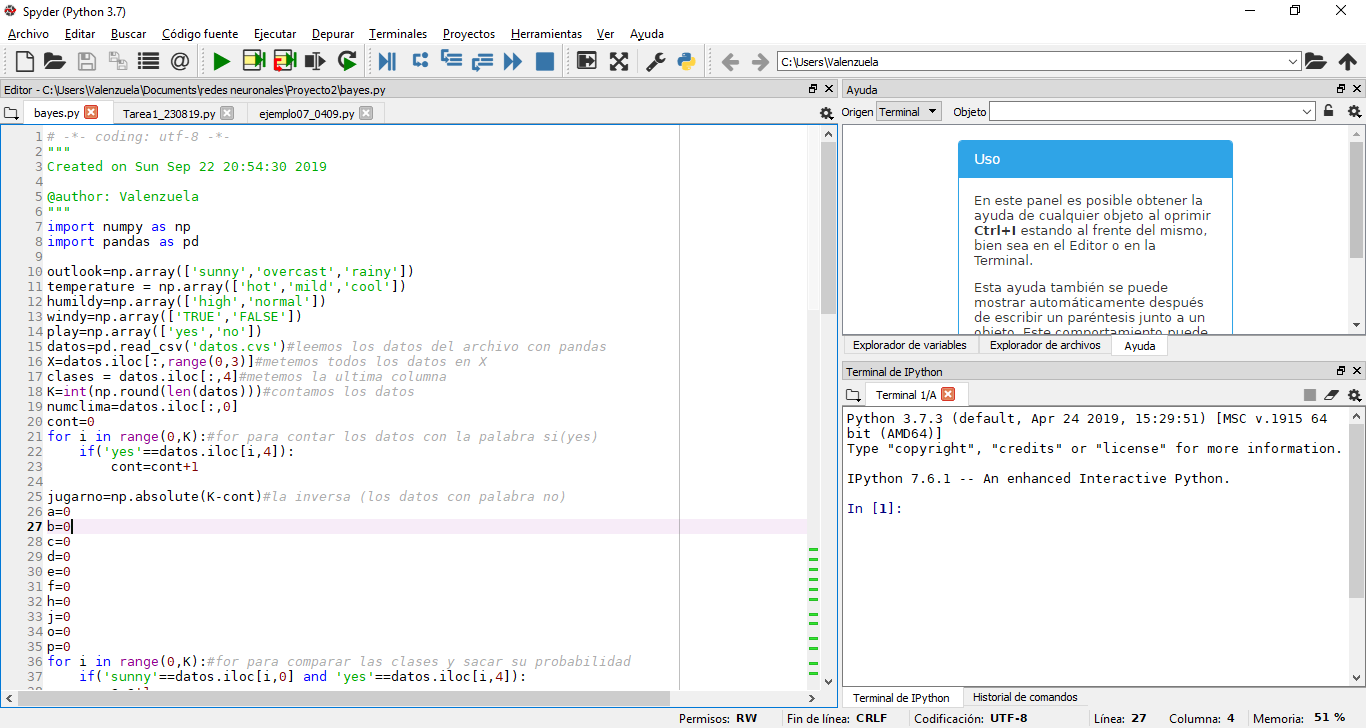
\includegraphics[scale=0.3] {codigo1.png}
\caption{Primer fragmento de codigo.}
\label{fig:Binarizacion}
\end{figure}

\paragraph{Realice un for para contar las veces que se repetia la palabra "yes" esto con la finalidad de obtener la probabilidad de clase esto se realizo simplemente comparando con iloc y la palabra "yes" todo esto dentro de un if.}

\paragraph{Una vez hecho esto procedí a comparar la probabilidad de cada una de las clases , en total 5, otra vez apoy\'andome de la ayuda de iloc y comparando con sus respectivos nombres, el resultado se dividi\'o con el total de clases sacado anteriormente y as\'i ya tenia lista la precisi\'on de cada una de las clases, solo me hacia falta leer los nuevos datos y multiplicar las precisiones para obtener la precisi\'on total.}

\begin{figure}[h]
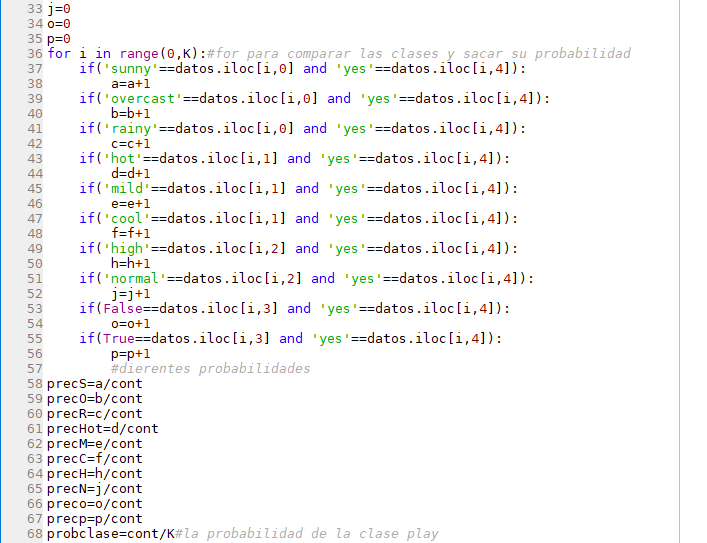
\includegraphics[scale=0.4] {codigo2.png}
\caption{Se muestra la comparacion de clases.}
\label{fig:Binarizacion}
\end{figure}

\paragraph{Para leer los datos de prueba cree otro archivo llamado datosprueba.cvs al igual que el anterior saque los datos gracias a iloc y obtuve los datos de la ultima clase, cont\'e el numero de filas y lo siguiente fue calcular la probabilidad de las clases para despu\'es poder multiplicarlas y obtener su valor.}

\paragraph{Guard\'e en diferentes arreglos los datos por columna para ir comparando los datos por filas por medio de un for e if, simplemente comparando el valor de los arreglos por sus respectivos posibles valores.}

\begin{figure}[h]
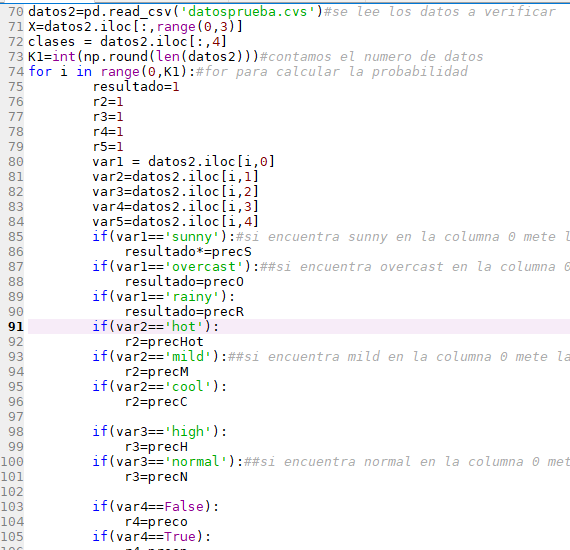
\includegraphics[scale=0.4] {codigo3.png}
\caption{Comparacion de datos por medio de los arreglos.}
\label{fig:Binarizacion}
\end{figure}

\paragraph{Para finalizar multiplique todos los resultados de las probabilidades encontradas dando como resultado la probabilidad de salir a jugar o no salir.}

\section{Conclusion}
\paragraph{El clasificador bayesiano es f\'acil de implementar y entender, al funcionar por medio de probabilidades podemos tener un muy buen entendimiento de este algoritmo, pudiendo calcular algunas series de datos para comprobar que el algoritmo funciona de manera correcta.
En conclusi\'on el clasificador bayesiano es muy bueno a la hora de predecir sucesos.}

\section{Referencias}
\paragraph{$http://www.ai.org.mx/ai/images/sitio/2014/05/ingresos/less/trabaj_final_dr._sucar.pdf$ Luis Enrique Sucar, Investigador Titular,Instituto Nacional de Astrofisica,Recuperado el 22 de Septiembre del 2019}

\end{document}